\begin{scanpage}{0124}{107}
\noindent\begin{minipage}[t]{.48\linewidth}\vspace{0pt}\centering
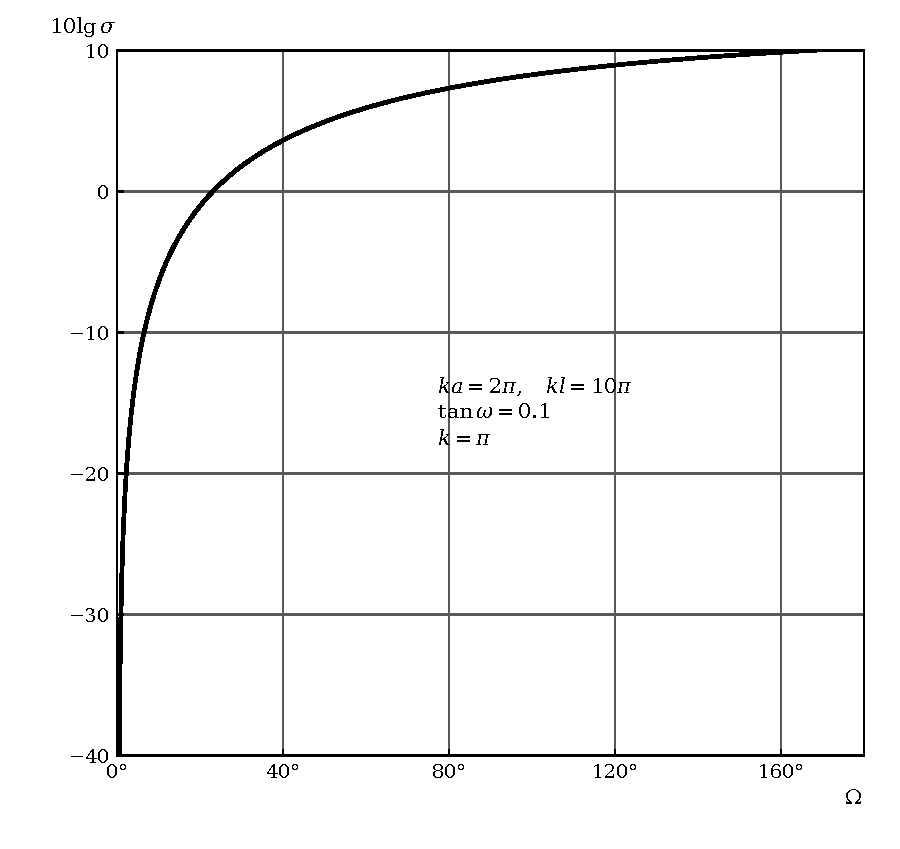
\includegraphics[width=.95\linewidth]{images/recreated/b-0124-fig39.pdf}

\raggedright Figure 39. The effective scattering area of a finite paraboloid as a function of the shape of the shaded part.
\end{minipage}\hfill\begin{minipage}[t]{.48\linewidth}\vspace{0pt}
In concluding this section, let us dwell for a moment on the question of calculating the effective scattering area for bodies of rotation of a complex shape, whose elements are the lateral surfaces of truncated paraboloids. The field from the nonuniform part of the current arising in the vicinity of circular discontinuities may be determined without difficulty from Equation (17.03). The field from the uniform part of the current is found by quadratures. Thus, the field being created in the direction $\vartheta=\pi$ by the uniform
\end{minipage}\par\medskip

part of the current which flows on the lateral surface of the truncated paraboloid $r^2=2pz$ $(p=a_1\operatorname{tg}\omega_1=a_2\operatorname{tg}\omega_2$; see Figure 40) is determined by the equation
\[\left.\begin{aligned}E_x=-H_y&=-\frac12E_{0x}(a_1\operatorname{tg}\omega_1-a_2\operatorname{tg}\omega_2e^{2ikl_2})e^{2ikl_1}\frac{e^{ikR}}R,\\E_y=H_x&=0.\end{aligned}\right\}\tag{18.07}\]
Here
\[l_2=\frac12(a_2\operatorname{ctg}\omega_2-a_1\operatorname{ctg}\omega_1)\tag{18.08}\]
is the height of the truncated paraboloid (the distance between its bases). Let us note that Equation (18.07) is a simple algebraic corollary of Expression (18.02): it is the difference of the fields scattered, respectively, by the paraboloid of height $l_1+l_2=\frac{a_2^2}{2p}$ and by the paraboloid of height $l_1=\frac{a_1^2}{2p}$.
\end{scanpage}
